% !TEX TS–program = pdflatexmk
% Specifies the compiler that will be used to generate the PDF.

\documentclass[a0,portrait]{a0poster} % A0 size poster
\usepackage[utf8]{inputenc} % Input encoding in UTF-8
\usepackage[backend=bibtex, style=numeric]{biblatex} % Bibliography
\DefineBibliographyStrings{english}{%
bibliography = {References}} % Change "Bibliography" to "References"
\addbibresource{references.bib} % Add bibliography from a .bib file

\usepackage{amsmath} % Mathematical package
\usepackage{amssymb} % Mathematical symbols
\usepackage{bbold} % Mathematical symbols font
\usepackage{amsthm} % Mathematical theorems
\usepackage{tikz}
\usepackage{cancel} % Cancel or strikethrough in mathematical equations

\usepackage{tikz}

\usepackage{cuted}
\usepackage{flushend}

\usepackage{amssymb} %maths%\usepackage{amsmath} %maths
\usepackage[utf8]{inputenc} %useful to type directly diacritic characters
\usepackage{feynmp-auto}

\usepackage{pgfplots}
\pgfplotsset{compat=1.8}

\usepackage{comment} % Comments
\usepackage[document]{ragged2e} % Alignment (justification)
\usepackage{multicol} % Multiple columns
\setlength{\columnsep}{3cm}

\usepackage[hidelinks]{hyperref} % Hyperlinks, with hidden links

\title{\textbf{\Huge Fierz-Pauli Field Theory}} % Title
\author{\textsc{\huge Juan José Fernández Morales}} % Author
\date{} % No date displayed


\usepackage{xcolor}

\pagecolor{black} % Bacground
\color{white} % Words colors
\pagestyle{empty} % No page number
\pagenumbering{gobble} % remove page numbering

\usepackage[pages=all]{background}
% configuración
\backgroundsetup{
 scale=1, %escala de la imagen, es recomendable que sea del mismo tamaño que el pdf
 color=black, %fondo a usar para transparencia
 opacity=0.4, %nivel de transparencia
 angle=0, %en caso de querer una rotación
 contents={%
  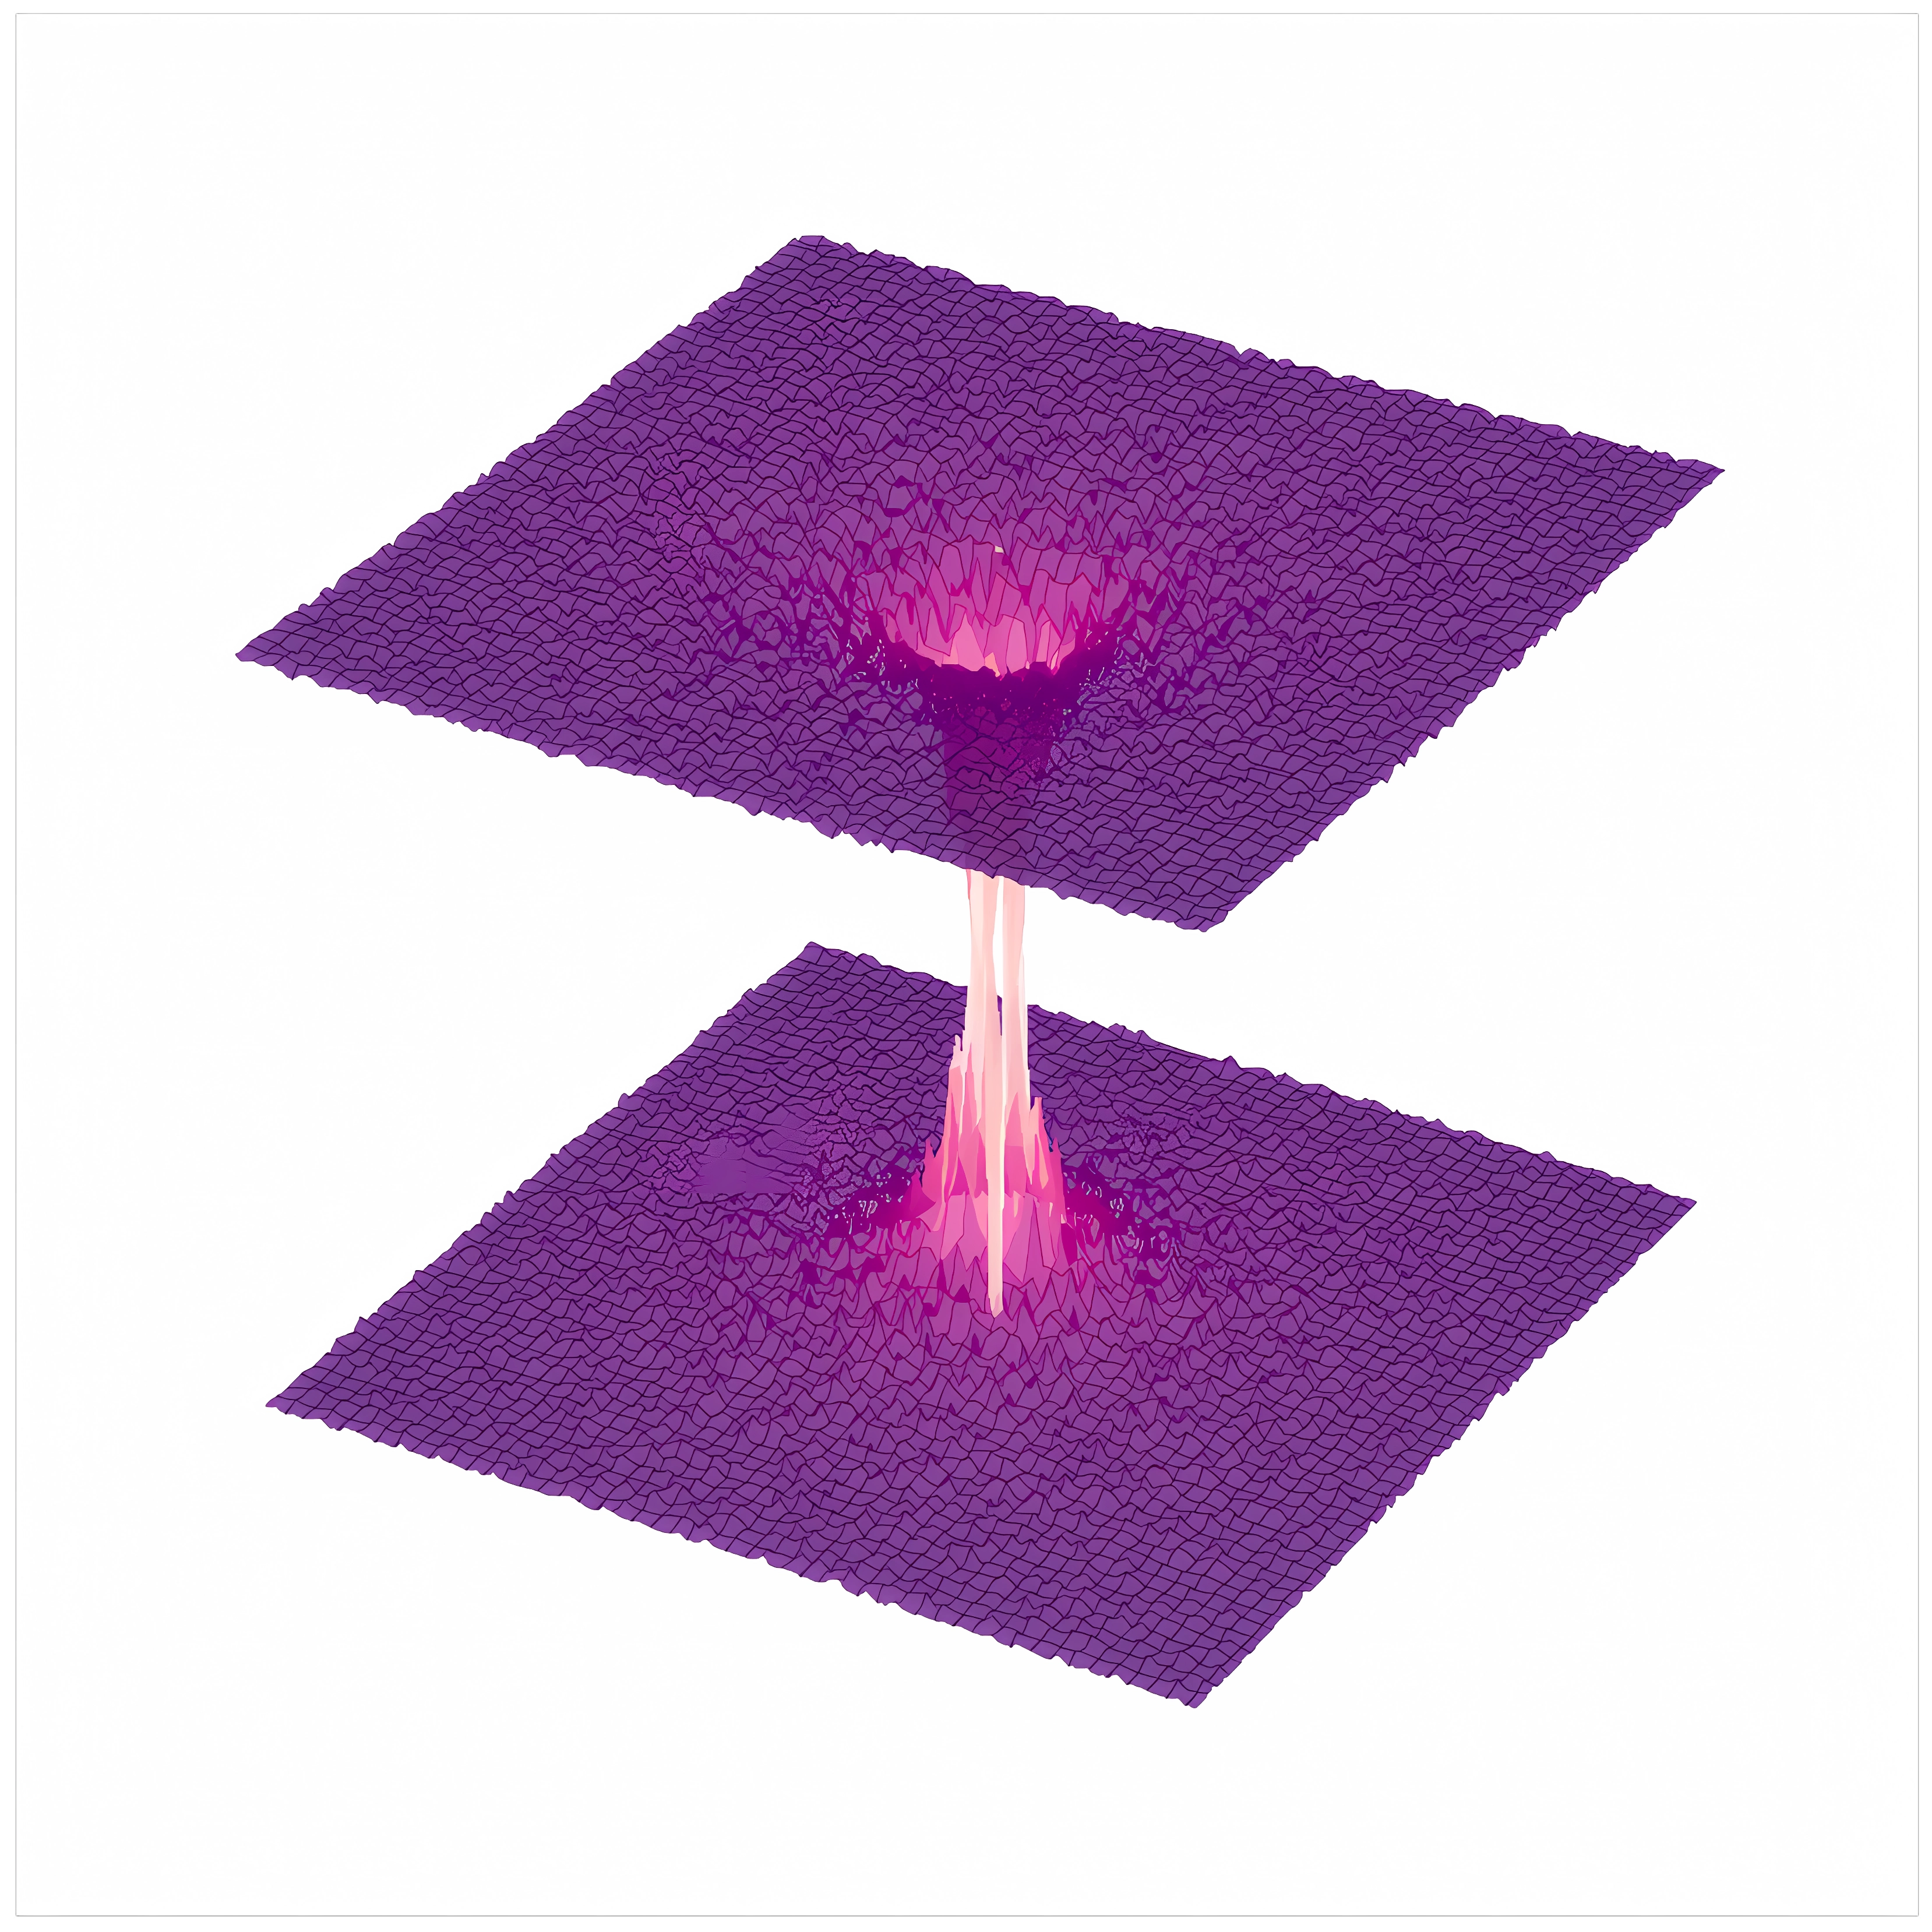
\includegraphics[width=180cm,height=160cm]{media/Background.png} %nombre de la imagen a utilizar como fondo
 }%
}

\begin{document}

%%%%%%%%%%%%%%%%%%%%%%%%%%%%%%%%%%%%%%%%%%%%%%%%%%%%%%%%%%%%%%%%%%%%%%%%%%
% CABECERA
\maketitle % Generate document title
%%%%%%%%%%%%%%%%%%%%%%%%%%%%%%%%%%%%%%%%%%%%%%%%%%%%%%%%%%%%%%%%%%%%%%%%%%
\begin{center}\Large
This poster presents a theory that explains how massless particles with spin 2 behave. We start by explaining why we choose a field, and why they are related with a spin, and then we move on to discussing the Fierz-Pauli Field Theory, which is a the only ghost-free model for a spin-2 field. We also show how this theory is related to Einstein's theory of gravity and how it can help us better understand the fundamental forces of the universe.% ABSTRACT
\end{center}

\vspace{1cm}

%%%%%%%%%%%%%%%%%%%%%%%%%%%%%%%%%%%%%%%%%%%%%%%%%%%%%%%%%%%%%%%%%%%%%%%%%%
% PRIMERA PARTE
\begin{multicols}{2}
%%%%%%%%%%%%%%%%%%%%%%%%%%%%%%%%%%%%%%%%%%%%%%%%%%%%%%%%%%%%%%%%%%%%%%%%%%

%%%%%%%%%%%%%%%%%%%%%%%%%%%%%%%%%%%%%%%%%%%%%%%%%%%%%%%%%%%%%%%%%%%%%%%%%%
\begin{center}
\section{Spin Field Theory} % INTRODUCTION
\end{center}
%%%%%%%%%%%%%%%%%%%%%%%%%%%%%%%%%%%%%%%%%%%%%%%%%%%%%%%%%%%%%%%%%%%%%%%%%%
\justify{\Large
Field theory provides a coherent and consistent explanation for physical interactions. Spin is a fundamental property of fields in physics, characterized by relativistic systems that determine field transformations under rotations. Understanding spin is crucial for comprehending field behavior in different reference frames.}

\begin{equation}
	\Large
	\phi_{A} = \phi_{A}(x_0, x_1, x_2, x_3) \equiv \phi_{A}(x).
\end{equation}

\justify{\Large Helicity $\xi$ can be described mathematically:}

\begin{equation}
	\Large
	\phi_{A}' = e^{i \xi \theta} \phi_{A},
\end{equation}

\justify{\Large where $\phi_{A}$ and $\phi_{A}'$ are the original and rotated field, respectively; $h$ is the helicity of each component of the vector and $\theta$ is the rotation angle.}

\hfill

\begin{center}
\begin{tikzpicture}[scale=3]
  \begin{axis}[
      axis lines=center,
      view={140}{25},
      axis equal,
      domain=0:360,
      y domain=0:1.1,
      xmax=1.5,ymax=1.5,zmin=0,zmax=1.5,
      x label style={at={(axis description cs:0.12,0.20)},anchor=north},
      y label style={at={(axis description cs:0.82,0.20)},anchor=north},
      z label style={at={(axis description cs:0.55,0.93)},anchor=north},
      label style={font=\tiny},
      xlabel = $x_{1}$,
      ylabel=$x_{2}$,
      zlabel=$\phi_{A}(x)$,
      ticks=none,
      clip bounding box=upper bound
    ]
    \addplot3 [surf, shader=flat, draw=black, fill=white, z buffer=sort] ({sin(x)*y}, {cos(x)*y}, {(y^2-1)^2});
 
 	 % add the curve arrow
    \addplot3 [white, thick, domain=90:300, samples=100, samples y=0, -latex] ({sin(x)}, {cos(x)}, 0.8) node [pos=0.9, above right, scale=0.5] {$\theta$} ;
  \end{axis}
\end{tikzpicture}
\end{center}

\justify{\Large Spin field theory plays a crucial role in understanding particles with integer spin and has been vital for the development of various areas of physics.}

%%%%%%%%%%%%%%%%%%%%%%%%%%%%%%%%%%%%%%%%%%%%%%%%%%%%%%%%%%%%%%%%%%%%%%%%%%
\begin{center}
\section{Fierz-Pauli Action}
\end{center}
%%%%%%%%%%%%%%%%%%%%%%%%%%%%%%%%%%%%%%%%%%%%%%%%%%%%%%%%%%%%%%%%%%%%%%%%%%


\justify{\Large The Fierz-Pauli action describes the dynamics of a spin-2, massless, symmetric, second-order tensor field $h_{\mu\nu}$. This action must satisfy the principles of locality and relativity. To capture the behavior of this field, we use the unique general ghost free Lagrangian \cite{Juanjo} that satisfies these characteristics can be expressed as:}

\begin{equation} 
	\large
	S_{FP} = 
	\int_{M_{4}} dx^{4} \left( \frac{1}{4} \partial_{\mu} h_{\nu\rho}\, \partial^{\mu}h^{\nu\rho}  
					    -\frac{1}{2}\, \partial_{\mu} h_{\nu\rho}\, \partial^{\nu}h^{\rho\mu} +
					     \frac{1}{2}\, \partial_{\mu} h\, \partial_{\rho}\, h^{\mu\rho} 
					    -\frac{1}{4}\, \partial_{\mu} h\, \partial^{\mu}h. \right),
\end{equation}

\justify{\Large where $h = \eta^{\mu\nu}h_{\mu\nu}$ and $M_{4}$ is the four-dimensional Minkowski space-time.}

\justify{\Large This Lagrangian is invariant under a gauge transformation}

\begin{equation}
	\Large
	S_{FP} \left(h_{\mu\nu}\right) = 
	S_{FP} \left( h'_{\mu\nu} = h_{\mu\nu} + \partial_\mu \xi_\nu + \partial_\nu \xi_\mu \right).
\end{equation}

\justify{\Large This characteristic is important because it allows us to choose a particular gauge that simplifies calculations. One common choice of gauge is the harmonic gauge, which is defined by the condition}

\begin{equation} \label{eq:gauge_election}
	\large
	\partial^{\mu}h_{\mu\nu} - \frac{1}{2}\partial_{\nu}h = 0.
\end{equation} 

\justify{\Large Furthermore, the choice of a full gauge allows the reduction of the degrees of freedom of the field, to such an extent that it matches the values expected by the Wigner classification. }

\justify{To obtain the equation of motion, we vary the action with respect to $h_{\mu\nu}$}

\begin{equation} \label{eq:eom}
	\Large
	\frac{ \delta S_{FP} }{ \delta h^{\mu\nu} } = 0 \land \eqref{eq:gauge_election}
	\hspace{5mm} \Longrightarrow \hspace{5mm}
	\partial_{\alpha}\partial^{\alpha}h_{\mu\nu} = 0.
\end{equation}

\justify{\Large This traceless solution for $h_{\mu\nu}$ is in accordance with a relativistic wave equation.}

\end{multicols}

\vspace{2cm}

%%%%%%%%%%%%%%%%%%%%%%%%%%%%%%%%%%%%%%%%%%%%%%%%%%%%%%%%%%%%%%%%%%%%%%%%%%
% SEGUNDA PARTE

%%%%%%%%%%%%%%%%%%%%%%%%%%%%%%%%%%%%%%%%%%%%%%%%%%%%%%%%%%%%%%%%%%%%%%%%%%

%%%%%%%%%%%%%%%%%%%%%%%%%%%%%%%%%%%%%%%%%%%%%%%%%%%%%%%%%%%%%%%%%%%%%%%%%%
\begin{center}
\section{Linear General Relativity} % GR LINEAL
\end{center}
%%%%%%%%%%%%%%%%%%%%%%%%%%%%%%%%%%%%%%%%%%%%%%%%%%%%%%%%%%%%%%%%%%%%%%%%%%
\begin{multicols}{3}
\begin{center}
\subsection*{General relativity}
\end{center}
% Primera columna
\justify{\Large The Einstein-Hilbert action (EHA) encapsulates the principles of general relativity, representing spacetime dynamics via geometry (see more in \cite{carroll2004spacetime}). It is given by:}

\begin{equation}
	\large
	S_{EH} \left( g_{\mu\nu} \right) =
	\frac{1}{16\pi G}\int_{\mathcal{M}_{4}}\mathrm{d}^4x\sqrt{\left| det(g_{\mu\nu}) \right| }R \left( g_{\mu\nu} \right),
\end{equation}

\justify{\Large where $g_{\mu\nu}$, $R$, and $G$ denote the metric tensor, scalar curvature, and gravitational constant, respectively. Einstein's field equation is derived from Einstein-Hilbert and material action using the Hamiltonian principle:}

\begin{equation}
\large
\frac{\delta \left(S_{EH} + S_{\text{material}} \right)}{\delta g^{\mu\nu}} = 0
\hspace{3mm} \Longrightarrow \hspace{3mm}
R_{\mu\nu} - \frac{1}{2}g_{\mu\nu} R=8\pi T_{\mu\nu}.
\end{equation}

\justify{\Large Here, $S_{\text{material}}$ represents the action of the rest of the physical system and $T_{\mu\nu}$ its stress-energy tensor, and $R_{\mu\nu}$ is the Ricci tensor.}

\vfill\null
\columnbreak

% Segunda columna
\begin{center}
\subsection*{General relativity - Spin-2}
\end{center}
\justify{\Large Consider a small fluctuation $h_{\mu\nu}$ around the Minkowski metric $\eta_{\mu\nu}$ \cite{Manoukian:2016jpj} as:}

\begin{equation}
\Large
g_{\mu\nu} = \eta_{\mu\nu} + \varepsilon h_{\mu\nu} \quad \downarrow  \quad \varepsilon^{3} \simeq 0,
\end{equation}

\justify{\Large Using this expression, we can re-express the elements of the Einstein-Hilbert action in terms of $h_{\mu\nu}$:}

\begin{align}
	\Large
	g^{\mu\nu} &=
	 \eta^{\mu\nu} - \varepsilon h^{\mu\nu} + \varepsilon^{2}h^{\mu\lambda}h_{\lambda}^{\nu} +  \mathcal{O}(\varepsilon^3), \\
	\sqrt{\left| det(g_{\mu\nu}) \right| } &= 
	1 +  \frac{\varepsilon}{2}h + \frac{\varepsilon}{8}h^{2} - \frac{\varepsilon^2}{4}h_{\mu\nu}h^{\mu\nu} + \mathcal{O}(\varepsilon^3), \\
	R\left( g_{\mu\nu} \right) &= \frac{1}{2} \left( \varepsilon R^{(1)} + \varepsilon^{2} R^{(2)} \right)+ \mathcal{O}(\varepsilon^3),
\end{align}

\justify{\Large where $h$ is the trace of the metric perturbation and the  $R^{(1)}$ and $R^{(2)}$ expression are:}

\begin{align*}
	R^{(1)}(\varepsilon) &=  \left( \eta^{\mu\nu} - \varepsilon h^{\mu\nu} \right) \left( \partial^{\rho}\partial_{\mu}h_{\nu\rho} + \partial^{\rho}\partial_{\nu}h_{\mu\rho} - \partial_{\alpha}\partial^{\alpha} h_{\mu\nu} - \partial_{\mu}\partial_{\nu}h \right), \\
	R^{(2)}(\varepsilon^2) &= \frac{1}{2}\,\partial_{\rho}h\partial^{\rho}h - \partial_{\lambda}h\partial_{\rho} h^{\rho\lambda} + \partial_{\rho}h_{\sigma\lambda}\partial^{\sigma}h^{\rho\lambda} - \frac{1}{2}\,\partial_{\rho}h_{\sigma\lambda}\partial^{\rho}h^{\sigma\lambda}.
\end{align*}

%R_{\mu\nu} \left( g_{\mu\nu} \right) &= 
%	\frac{\varepsilon}{2} \left( \partial^{\rho}\partial_{\mu}h_{\nu\rho} + \partial^{\rho}\partial_{\nu}h_{\mu\rho} - \partial_{\alpha}\partial^{\alpha} h_{\mu\nu} - \partial_{\mu}\partial_{\nu}h \right)+ \\
%	& \frac{\varepsilon^2}{2} \left( \partial_{\lambda}h_{\mu\nu}\partial_{\rho} h^{\rho\lambda} - \frac{1}{2}\partial_{\rho}h\partial^{\rho}%h_{\mu\nu} - \frac{1}{4}\eta_{\mu\nu}\partial_{\rho}h_{\sigma\lambda}\partial^{\sigma}h^{\rho\lambda}  + \frac{1}{8}\eta_{\mu\nu}\partial_{\rho}h_{\sigma\lambda}\partial^{\rho}h^{\sigma\lambda} \right)+ \mathcal{O}(\varepsilon^3) \\

\justify{\Large Using the expressions above, we can write the perturbative Lagrangian as:}

\vfill\null
\columnbreak

% Fluctuación lineal de la métrica, consecuencia para el tensor escalar de Ricci, y para el determinante
% Substitution and FP
\begin{center}
\subsection*{Newton - Spin-2}
\end{center}
% Tercera columna, Efective potential, diagram one loop feymann
\justify{\Large By choosing the harmonic gauge \eqref{eq:gauge_election}, the equation of motion of $h_{\mu\nu}$ this perturbative action takes the form:}

\begin{equation}
	\Large
	\partial_{\alpha}\partial^{\alpha} h_{\mu\nu} = -\frac{1}{\kappa^{2}} \left( T_{\mu\nu} - \frac{1}{2}\eta_{\mu\nu}T \right).
\end{equation}
s
\justify{\Large In the non-relativistic limit, the energy-momentum tensor for a static particle of mass $M$ can be described like:}

\begin{equation}
	\Large
	T_{\mu\nu} = \varepsilon^{2} M \, \delta_{\mu}^{0} \, \delta_{\nu}^{0} \, \delta(\vec{x}),
\end{equation}

\justify{\Large where the first two deltas are Kronecker deltas, and the third one is a Dirac delta for the spatial coordinates. Solving the equation of motion \cite{Hinterbichler:2011tt} we obtain:}

\begin{equation}
	\Large
	h_{00} = \frac{1}{4 \kappa^{2}}\frac{\varepsilon^{2}M}{r} = \frac{2GM}{r},
\end{equation}

\justify{\Large the gravitational potential of Newton's Law.}

\end{multicols}

\begin{align*}
\Large
\mathcal{L}_{EH} \left( \eta_{\mu\nu} + \varepsilon h_{\mu\nu} \right) &\simeq
\varepsilon^{2}\left( \frac{1}{4} \partial_{\mu} h_{\nu\rho}\, \partial^{\mu}h^{\nu\rho}  
					    -\frac{1}{2}\, \partial_{\mu} h_{\nu\rho}\, \partial^{\nu}h^{\rho\mu} +
					     \frac{1}{2}\, \partial_{\mu} h\, \partial_{\rho}\, h^{\mu\rho} 
					    -\frac{1}{4}\, \partial_{\mu} h\, \partial^{\mu}h \right),  \\
&\therefore S_{EH} \left( \eta_{\mu\nu} + \varepsilon h_{\mu\nu} \right) \simeq \kappa^{2} S_{FP}, \quad \kappa^{2} = \frac{ \varepsilon^{2} }{ 16\pi G }
\end{align*}

\justify{\Large \textbf{Peering into the abyss of quantum gravity, we stand at the precipice of unfathomable revelations that may shatter our comprehension of the cosmos. Delving into this enigmatic domain could unlock the deepest mysteries of existence, rewriting our understanding of reality itself.}}

\begin{tikzpicture}[remember picture,overlay]
\node[anchor=south east, inner sep=14pt] at ([xshift=-3.5cm]current page.south east) {\includegraphics[width=18cm]{media/logo_coefis_blanco.png}};
\end{tikzpicture}

\vspace{3cm}

\printbibliography[heading=bibintoc] 

\end{document}
